\section{Krav}

Indledning til kapitlet

\subsection{Systembeskrivelse}

\textit{På nuværende tidspunkt anvendes SCG kun til forskningsbrug og SCG til hjemmemonitorering er derfor endnu ikke implementeret \ref{}. På grund af dette, er der behov udarbejdelsen af et forskningsprojekt som undersøger, om SCG er en brugbar metode til hjemmemonitorering af hjertesvigtspatienter. Formålet med dette projekt er derfor at udvikle et prototype-system, som skal anvendes i forbindelse med et tilsvarende forskningsprojekt. I det følgende vil de forskellige dele af systemet blive beskrevet mere detaljeret.}

Systemet består af tre dele dele: en forskningsdatabase, et brugersystem og et administrerende system. Forskningsdatabasens primære formål er at lagre brugerdata, som skal anvendes til videre forskning. Derudover indeholder forskningsdatabasen login informationer for både bruger og administrator. Brugersystemet udvikles som en app, der anvendes af brugeren, mens det administrerende system anvendes af autoriserede personer, som skal have tilgang til forskningsdatabasen samt oprette bruger/administrator-profiler. \\
App'en skal kunne benyttes af brugeren i eget hjem uden opsyn af sundhedsfagligt personale og skal kunne måle SCG med et accelerometer, som er tilgængeligt i brugeren smartphone. Da der er tale om data som skal anvendes til forskningsbrug, vil brugeren blive anonymiseret og den enkelte bruger registreres derfor med brugerID og NYHA-klasse. Brugen af NYHA-klasser anvendes, da sværhedsgraden af hjertesvigtspatienters symptomer varierer alt efter hvilken NYHA-klasse de befinder sig i jvf. afsnit \ref{dentidligefase}. Dette kan have en indvirkning på brugerens SCG-måling, som man i en viderebehandling af data kan tage forbehold for. For at sikre kvaliteten af SCG-signalet foretages målingen med brugeren i liggende position. Dette sikrer at smartphonen kan ligge på brystkassen, og at støj fra bevægelse mindskes. \\
%Parametrene alder og køn kan være nyttige ift. indsamling af statistik. 
Da hjertesvigt hyppigst rammer den ældre befolkning, skal systemet være brugervenligt og tage hensyn til denne patientgruppe. Vejledninger skal derfor stå med let læselig tekst, illustreres med billeder og desuden læses op. Der skal ligeledes være et begrænset antal knapper som skal være store. Desuden skal knapperne understøttes både visuelt og auditivt. Når brugeren trykker på knappen, skal dennes funktion læses op og hvis brugeren er enig så skal de trykke igen. \\
Der foretages en måling hver 7. dag. Denne målingsfrekvens er fastsat på baggrund af et studie foretaget af \citet{teleprog} jvf. afsnit \ref{telemonitoreringhjertesvigt}. Dette tidsinterval hænger desuden også sammen med afsnit \ref{praudskrivelse} hvor den første lægekonsultation efter udskrivelsen ifølge \cite{Yancy2013} bør finde sted 7 til 14 dage efter udskrivelsen. \\
Compliance er en udfordring for de ældre jvf. afsnit \ref{forebyggelse}. Brugeren vil derfor modtage en notifikation, som skal påminde brugeren om at foretage en måling den pågældende dag. \\
Ifølge afsnit \ref{hjertesvigt} er der symptomer som kendetegner hjertesvigt. Brugeren skal i forbindelse med målingen udfylde et spørgeskema, der giver brugeren mulighed for at beskrive sine nuværende symptomer. Dette kan være brugbart i forbindelse med en evt. tolkning af data samt estimering af alarm parametre. Efter flere målinger er målet bl.a. at kunne koble hjertesvigtspatienternes symptomer på den målte SCG.\\
Der tages højde for sikkerhedsfunktioner idet både administratorsystemet og brugersystemet er passwordbeskyttet. I brugerens tilfælde sikrer dette, at det kun er den enkelte bruger som har mulighed for at foretage en måling og forveksling ikke finder sted. Desuden krypteres data, for at sikre at data ikke benyttes uautoriseret. Da data skal benyttes til forskningsmæssig brug, registreres brugerne ikke med navn eller CPR. Denne anonymitet giver samtidig også en form for patientsikkerhed. Yderligere skal brugerne automatisk logges af ved inaktivitet. Denne feature skal inkorporeres for både brugeren og administratoren. \\
SCG-målingerne kan påvirkes af artefakter og skal derfor filtreres før de bliver sendt videre til databasen. Dette indebærer artefakter associeret med hjertelyde, DC-offset og respirationsbevægelser, hvilket muliggør en estimering af brystkassebevægelser som repræsenterer det interesserede SCG-signal \citep{Wick2014}. Filtreret data gør det muligt at tjekke for fejlmålinger. Hvis der detekteres en fejlmåling forkastes målingen og brugeren skal bedes om at foretage en ny måling. I tilfælde af at mobilen tabes, skal målingen desuden afbrydes og startes forfra. Disse foranstaltninger skal bl.a. sikre at der ikke sendes unødige målinger.

\subsection{Use cases}

Systembekrivelsen bidrager til at systemets behov bliver identificeret samt grænserne for systemet sættes. Dette kan yderligere beskrives vha. use cases, som definerer hvad systemet skal kunne. Før det er muligt at definere use cases, skal aktørerne først identificeres. Aktørerne definerer hvem der interagerer med systemet mens hvad disse kan udføre defineres use cases. Use cases specificerer dermed de enkelte funktionaliteter som systemet besidder og har til formål at skabe et overblik over det samlede system.

\subsubsection{Use case diagram}
På baggrund af systembeskrivelsen er følgende use case diagram, jvf. figur \ref{fig:usecase}, udarbejdet. Denne viser sammenspillet mellem de enkelte use cases samt aktørerne i det samlede system. De enkelte use cases illustreres med en elipse samt et navn som tydeligt indikerer hvad den enkelte aktør kan udføre når denne interagerer med systemet. Som det fremgår af figur \ref{fig:usecase} identificeres to aktører, henholdvis bruger og administrator, som interagerer med hver deres system samt tilhørende brugergrænseflade. Disse to systemer interagerer ikke indbyrdes mellem hinanden, hvilket er illustreret ved at det enkelte system er afgrænset i en ramme/boks. De to systemer interagerer til gengæld med hinanden gennem en forskningsdatabase, hvor det er muligt at lagre og hente data fra de respektive systemer. Relationen mellem aktør og use case indikeres med en linje som forbinder disse to. En use case kan også være i forlængelse af en anden use case som indikeres med stiplede linjer enten kombineret med <<extends>> eller <<includes>>, hvortil pilen peger hen mod den use case den tilhører. Forskellen på disse er at <<includes>> er obligatorisk mens <<extends>> ikke er, sidstnævnte kan dermed betragtes som en ekstrafunktion som kan anvendes efter behov.      

\begin{figure}[H]
\centering
  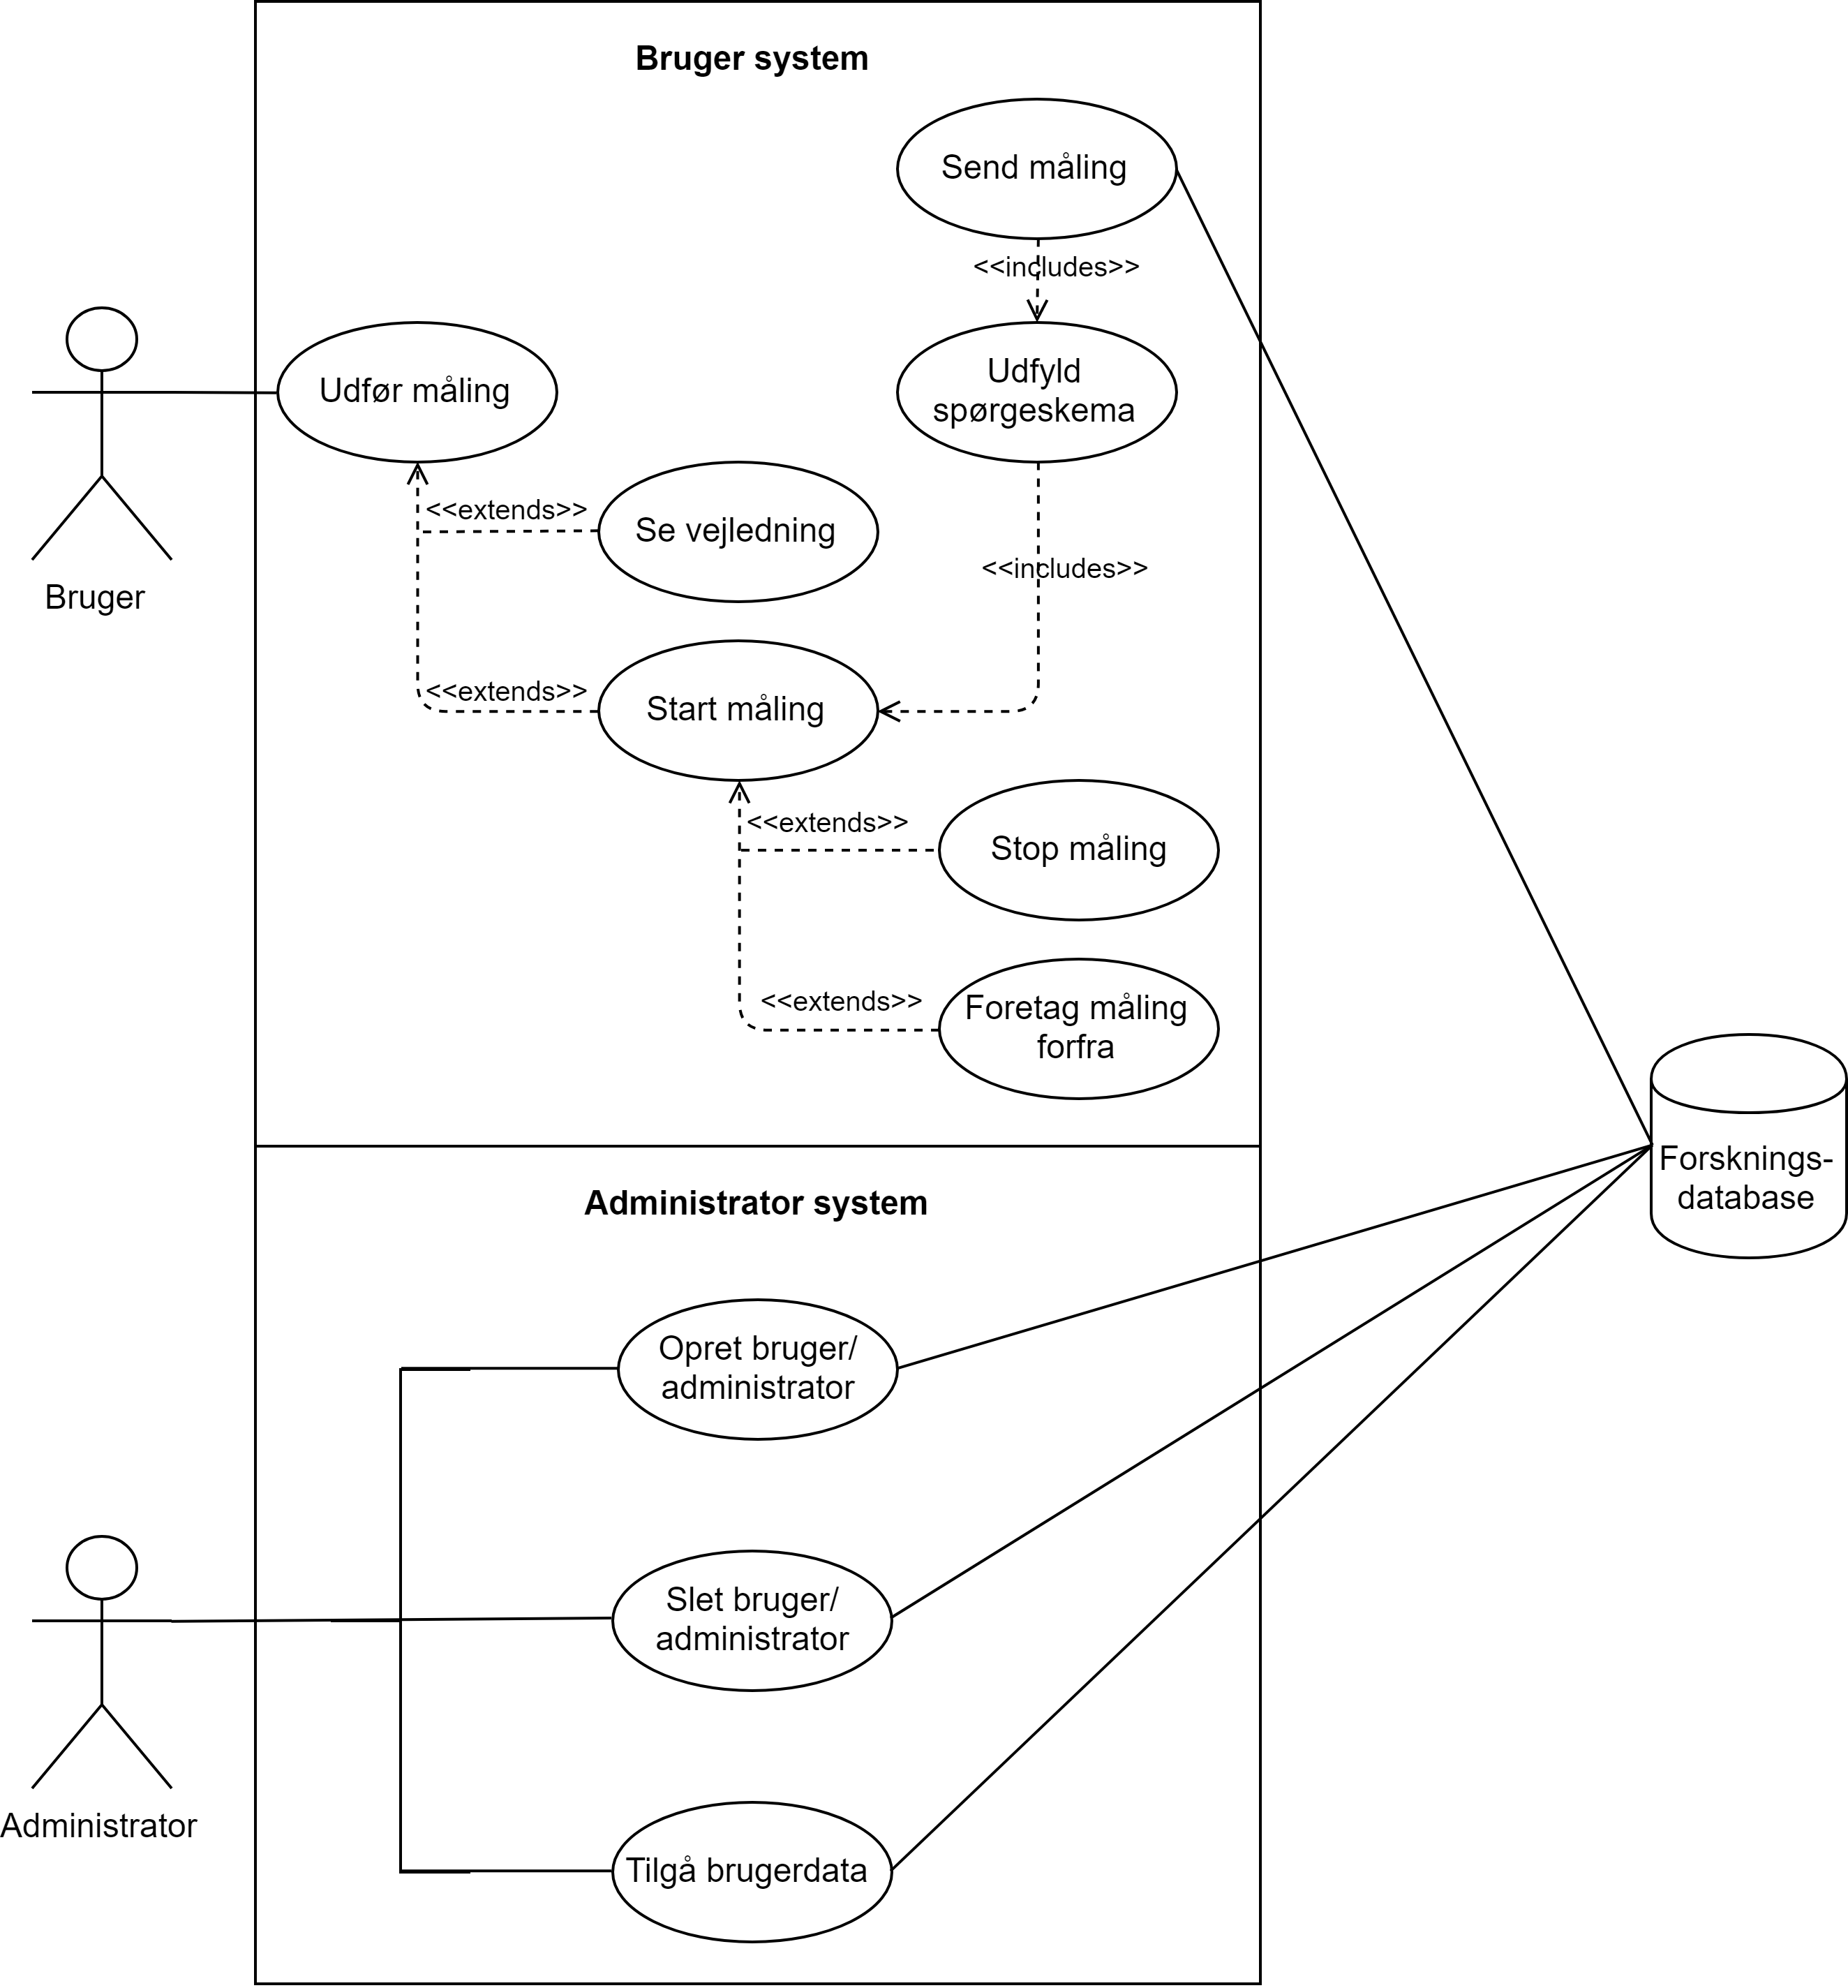
\includegraphics[width=1\textwidth]{Billeder/Usecase.png}
   \caption{Use case diagram for et system som kan måle SCG hos hjertesvigtspatienter og opsamle data i en forskningsdatabase i forbindelse med et forskningsprojekt. } 
   \label{fig:usecase}
\end{figure}

\subsubsection{Use case beskrivelser}
Ud fra use case diagrammet er der udarbejdet nogle use case beskrivelser. Disse har til formål at beskrive de enkelte use cases mere i dybden, hvortil følgende beskrives:

\begin{itemize}
    \item \textit{Aktører} definerer hvem der kan udføre den pågældende use case.
    \item \textit{Startbetingelser} definerer de forudsætninger som skal være opfyldt forud for at en use case kan initieres.
    \item \textit{Udløser} definerer begivenheder som initierer den pågældende use case.
    \item \textit{Normaltilstand} er en trin for trin beskrivelse af alle de aktiviteter som er nødvendige for at den pågældende use case udføres korrekt.
    \item \textit{Undtagelser} beskriver den eller de tilstande som afviger fra normaltilstanden samt det efterfølgende forløb.
\end{itemize}

I det følgende præsenteres først de beskrivende use cases for brugersystemet, hvorefter administrator systemet præsenteres. Brugersystemet indeholder én overordnet use case, 'Udfør måling', hvortil andre use cases kan tilgåes som forlængelse af denne. Disse kan enten være i form af included eller extended use cases. I første omgang henvises der blot til disse use cases under relevante trin i normaltilstand i use casen 'Udfør måling', efterfølgende uddybes disse i deres egen beskrivende use cases.  
%%%Udfør måling
\begin{table}[H]
\centering
\begin{tabular}{|l|}
\hline
\multicolumn{1}{|c|}{ \textbf{Use case 'Udfør måling'}}                                                                                                                                                                                                                                                                                                                                                                                                                                                                                                                                                                                       \\ \hline
\begin{tabular}[c]{@{}l@{}}\textbf{Aktører}\\ Bruger\end{tabular}                                                                                                                                                                                                                                                                                                                                                                                                                                                                                                                                                           \\ \hline
\begin{tabular}[c]{@{}l@{}} \textbf{Startbetingelser}\\ Bruger er oprettet i systemet\end{tabular}                                                                                                                                                                                                                                                                                                                                                                                                                                                                                                                           \\ \hline
\begin{tabular}[c]{@{}l@{}} \textbf{Udløser}\\ Bruger åbner app\end{tabular}                                                                                                                                                                                                                                                                                                                                                                                                                                                                                                                                                 \\ \hline
\begin{tabular}[c]{@{}l@{}} \textbf{Normaltilstand}\\ 1. Bruger logger ind \\    \hspace{3mm} 1.1 Bruger indtaster sit brugerID samt password\\  \hspace{3mm}   1.2 Brugerens oplysninger verificeres \\ 2. Systemet skal give brugeren et overblik over de forskellige valgmuligheder\\    \hspace{3mm} 2.1. Bruger trykker på extension 'Start måling'\\   \hspace{3mm}  2.2. Bruger trykker på extension 'Se vejledning'\\ 3. Data tjekkes for fejlmåling samt filtreres\\ 4. Data godkendes\\ 5. Include(Udfyld spørgeskema)\\ 6. Include(Send data)\\ 7. Systemet skal fortælle brugeren at der er foretaget en succescfuld måling\\ 8. Bruger logger af\end{tabular} \\ \hline
\begin{tabular}[c]{@{}l@{}} \textbf{Undtagelser}\\ 1 a) Brugerens oplysninger kan ikke verificeres \\   \hspace{3mm} - Returner fejlmeddelelse at brugerID og/eller password er forkert og \\  \hspace{6mm}    vend tilbage til trin 1.1\\ 2 a) Brugere kan ikke trykke på knapper \\ \hspace{3mm}   - Returner fejlmeddelelse og bed brugeren om at genstarte sin app\\ 3 a) Der detekteres en fejlmåling og data godkendes ikke\\  \hspace{3mm}  - Returner fejlmeddelelse og vend tilbage til trin 2\end{tabular}                                                                                                                                                         \\ \hline
\begin{tabular}[c]{@{}l@{}} \textbf{Alternativ tilstand}\\ Ved 5 minutters inaktivitet logges brugeren af\end{tabular}                                                                                                                                                                                                                                                                                                                                                                                                                                                                                                       \\ \hline
\end{tabular}
\caption{Use case beskrivelse af 'Udfør måling'}
\label{my-label}
\end{table}
%%%%Start måling
\begin{table}[H]
\centering
\begin{tabular}{|l|}
\hline
\multicolumn{1}{|c|}{\textbf{Extension use case 'Start måling'}}                                                                                                                       \\ \hline
\begin{tabular}[c]{@{}l@{}} \textbf{Extends}\\ 'Udfør måling'\end{tabular}                                                                                                                       \\ \hline
\begin{tabular}[c]{@{}l@{}} \textbf{Normaltilstand} \\ 1. Systemet tilgår accelerometer i brugerens smartphone\\ 2. Systemet optager data \\ 3. Data lagres på brugerens smartphone\end{tabular} \\ \hline
\begin{tabular}[c]{@{}l@{}} \textbf{Undtagelser}\\ 1 a) 2 a) eller 3 a) virker ikke efter hensigten \\ \hspace{3mm} - Returner fejlmeddelelse og bed brugeren om at genstarte sin app\end{tabular}                                                          \\ \hline
\end{tabular}
\caption{Extension use case beskrivelse af 'Start måling'}
\label{my-label}
\end{table}
%%%%se måling

\begin{table}[H]
\centering
\begin{tabular}{|l|}
\hline
\multicolumn{1}{|c|}{\textbf{Extension use case 'Se vejledning'}}                                                                                                        \\ \hline
\begin{tabular}[c]{@{}l@{}} \textbf{Extends}\\ 'Udfør  måling'\end{tabular}                                                                                                         \\ \hline
\begin{tabular}[c]{@{}l@{}} \textbf{Normaltilstand} \\ 1. Systemet starter en vejledning \\ 2. Bruger ser vejledning\end{tabular} \\ \hline
\begin{tabular}[c]{@{}l@{}} \textbf{Undtagelser}\\ 1 a) virker ikke efter hensigten \\ \hspace{3mm} - Returner fejlmeddelelse og bed brugeren om at genstarte sin app\end{tabular}                                            \\ \hline
\end{tabular}
\caption{Extension use case beskrivelse af 'Se vejledning'}
\label{my-label}
\end{table}
%%%%%%% Udfyld spørgeskema%%%%%%%%%%%%%%%%
\begin{table}[H]
\centering
\begin{tabular}{|l|}
\hline
\multicolumn{1}{|c|}{\textbf{Use case 'Udfyld spørgeskema'}}                                                                                                           \\ \hline
\begin{tabular}[c]{@{}l@{}} \textbf{Aktør}\\ Bruger\end{tabular}                                                                                                                 \\ \hline
\begin{tabular}[c]{@{}l@{}} \textbf{Startbetingelser}\\ Målingen er godkendt\end{tabular}                                                            \\ \hline
\begin{tabular}[c]{@{}l@{}} \textbf{Udløser}\\ Bruger trykker på 'Udfyld spørgeskema'\end{tabular}                                                                                      \\ \hline
\begin{tabular}[c]{@{}l@{}} \textbf{Normaltilstand} \\ 1. Spørgeskema vises på brugergrænsefladen\\ 2. Bruger udfylder spørgeskema\end{tabular}                                  \\ \hline
\begin{tabular}[c]{@{}l@{}} \textbf{Undtagelser}\\ 1 a) eller 2 a) virker ikke efter hensigten \\ \hspace{3mm} - Returner fejlmeddelelse og bed brugeren om at genstarte sin app\end{tabular} \\ \hline
\end{tabular}
\caption{Use case beskrivelser af 'Udfyld spørgeskema'}
\label{my-label}
\end{table}

%%%%%%%%%%%send data%%%%%%%%%%%%%%%%%
\begin{table}[H]
\centering
\begin{tabular}{|l|}
\hline
\multicolumn{1}{|c|}{\textbf{Use case 'Send data'}}                                                                                                                                                                                                                                                                                                                                           \\ \hline
\begin{tabular}[c]{@{}l@{}} \textbf{Aktør}\\ Bruger\end{tabular}                                                                                                                                                                                                                                                                                                                                        \\ \hline
\begin{tabular}[c]{@{}l@{}} \textbf{Startbetingelser}\\ Bruger har udfyldt spørgeskema\end{tabular}                                                                                                                                                                                                                                                                                                     \\ \hline
\begin{tabular}[c]{@{}l@{}} \textbf{Udløser}\\ Bruger trykker på 'Send data'\end{tabular}                                                                                                                                                                                                                                                                                                               \\ \hline
\begin{tabular}[c]{@{}l@{}} \textbf{Normaltilstand} \\ 1. Systemet sender måling til databasen\\ 2. Systemet sender spørgeskema til databasen\\ 3. Systemet sender den pågældende tid og dato til databasen \\ 4. Systemet skal fortælle brugeren at data er sendt\end{tabular}                                                                                                                                                                                        \\ \hline
\begin{tabular}[c]{@{}l@{}} \textbf{Undtagelser}\\ 1 a) Måling kan ikke sendes\\ \hspace{3mm} - Returner fejlmeddelelse og bed brugeren om at foretage en ny måling\\ \hspace{3mm} - Vend tilbage til use case 'Udfør måling' trin 2 \\ 2 a) Spørgeskema kan ikke sendes \\ \hspace{3mm} - Returner fejlmeddelelse og bed brugeren om at udfylde spørgeskema på ny\\  \hspace{3mm} - Vend tilbage til extension use case 'Udfyld spørgeskema'\end{tabular} \\ \hline
\end{tabular}
\caption{Use case beskrivelse af 'Send data'}
\label{my-label}
\end{table}

%%%%%%%%%Opret adminstrator%%%%%%%%%%%%
\begin{table}[H]
\centering
\begin{tabular}{|l|}
\hline
\multicolumn{1}{|c|}{\textbf{Use case 'Opret administrator'}}                                                                                                                                                                                                                                      \\ \hline
\begin{tabular}[c]{@{}l@{}} \textbf{Aktør}\\ Administrator\end{tabular}                                                                                                                                                                                                                                             \\ \hline
\begin{tabular}[c]{@{}l@{}} \textbf{Startbetingelser}\\ Administrator systemet er åbnet\end{tabular}                                                                                                                                                                                                                        \\ \hline
\begin{tabular}[c]{@{}l@{}} \textbf{Udløser}\\ Administrator trykker på 'Opret administrator'\end{tabular}                                                                                                                                                                                                   \\ \hline
\begin{tabular}[c]{@{}l@{}} \textbf{Normaltilstand} \\ 1. Administrator udfylder informationer om den pågældende administrator\\ 2. Systemet verificerer at alle felter er udfyldt\\ 3. Administratorens oplysninger lagres i databasen\\ 4. Systemet fortæller at oprettelse er foretaget\end{tabular} \\ \hline
\begin{tabular}[c]{@{}l@{}} \textbf{Undtagelser}\\ 2 a) Der er tomme felter \\  \hspace{3mm}  - Fejlmeddelelser vises ved de tomme felter og vend tilbage til trin 1\\ 3 a) eller 4 a) virker ikke efter hensigten\\  \hspace{3mm} - Returner fejlmeddelelse og bed adminstrator om at genstarte sit system\end{tabular}               \\ \hline

\end{tabular}
\caption{Use case beskrivelse af 'Opret administrator'}
\label{my-label}
\end{table}

%%%%%%%%%%%%%Opret bruger %%%%%%%%%%%%%%%%%
\begin{table}[H]
\centering
\begin{tabular}{|l|}
\hline
\multicolumn{1}{|c|}{\textbf{Use case 'Opret bruger'}}                                                                                                                                                                                                                                      \\ \hline
\begin{tabular}[c]{@{}l@{}} \textbf{Aktør}\\ Administrator\end{tabular}                                                                                                                                                                                                                                             \\ \hline
\begin{tabular}[c]{@{}l@{}} \textbf{Startbetingelser}\\ 1. Administrator er opretttet i systemet \\ 2. Administrator er logget ind \end{tabular}                                                                                                                                                                                                                        \\ \hline
\begin{tabular}[c]{@{}l@{}} \textbf{Udløser}\\ Administrator trykker på 'Opret bruger'\end{tabular}                                                                                                                                                                                                   \\ \hline
\begin{tabular}[c]{@{}l@{}} \textbf{Normaltilstand} \\ 1. Administrator udfylder informationer om den pågældende bruger\\ 2. Systemet verificerer at alle felter er udfyldt\\ 3. Brugerens oplysninger lagres i databasen\\ 4. Systemet fortæller at oprettelse er foretaget\end{tabular} \\ \hline
\begin{tabular}[c]{@{}l@{}} \textbf{Undtagelser}\\ 2 a) Der er tomme felter \\  \hspace{3mm}  - Fejlmeddelelser vises ved de tomme felter og vend tilbage til trin 1\\ 3 a) eller 4 a) virker ikke efter hensigten\\  \hspace{3mm} - Returner fejlmeddelelse og bed adminstrator om at genstarte sit system\end{tabular}               \\ \hline
\begin{tabular}[c]{@{}l@{}} \textbf{Alternativ tilstand}\\ Ved 5 minutters inaktivitet logges administratoren af\end{tabular}                                                                                                                                                                                       \\ \hline
\end{tabular}
\caption{Use case beskrivelse af 'Opret bruger'}
\label{my-label}
\end{table}
%%%%%%%%%%%%%slet bruger %%%%%%%%%%%%%
\begin{table}[H]
\centering
\begin{tabular}{|l|}
\hline
\multicolumn{1}{|c|}{\textbf{Use case 'Slet administrator/bruger'}}                                                                                                                                                                                                                               \\ \hline
\begin{tabular}[c]{@{}l@{}} \textbf{Aktør}\\ Administrator\end{tabular}                                                                                                                                                                                                                                     \\ \hline
\begin{tabular}[c]{@{}l@{}} \textbf{Startbetingelser}\\ Administrator er logget på \end{tabular}                                                                                                                                                                                                                \\ \hline
\begin{tabular}[c]{@{}l@{}} \textbf{Udløser}\\ Administrator trykker på 'Slet bruger/administrator'\end{tabular}                                                                                                                                                                                            \\ \hline
\begin{tabular}[c]{@{}l@{}} \textbf{Normaltilstand} \\ 1. Systemet viser en oversigt over oprettede brugere/administratorer\\ 2. Administrator vælger den relevante bruger/administrator\\ 3. Administrator verificerer sit valg\\ 4. Den relevante bruger/administrator slettes fra databasen \\ 5. Systemet fortæller at oprettelse er foretage \end{tabular} \\ \hline
\begin{tabular}[c]{@{}l@{}} \textbf{Undtagelser}\\ 1 a) 2 a) 3 a) 4 a) virker ikke efter hensigten\\  \hspace{3mm} - Returner fejlmeddelelse og bed administrator om at genstarte sit system\end{tabular}                                                                                                        \\ \hline
\begin{tabular}[c]{@{}l@{}} \textbf{Alternativ tilstand}\\ Ved 5 minutters inaktivitet logges administratoren af\end{tabular}                                                                                                                                                                               \\ \hline
\end{tabular}
\caption{Use case beskrivelse af 'Slet bruger/administrator'}
\label{my-label}
\end{table}

%%%%%%%%%%%%%%tilgå brugerdata %%%%%%%%%%%%%
\begin{table}[H]
\centering
\begin{tabular}{|l|}
\hline
\multicolumn{1}{|c|}{\textbf{Use case 'Tilgå brugerdata'}}                                                                                                                                                                                                                                                                                                                   \\ \hline
\begin{tabular}[c]{@{}l@{}}\textbf{Aktør}\\ Administrator\end{tabular}                                                                                                                                                                                                                                                                                                     \\ \hline
\begin{tabular}[c]{@{}l@{}}\textbf{Startbetingelser}\\ Administrator er logget på\end{tabular}                                                                                                                                                                                                                                                                             \\ \hline
\begin{tabular}[c]{@{}l@{}}\textbf{Udløser}\\ Administrator trykker på 'Tilgå brugerdata'\end{tabular}                                                                                                                                                                                                                                                                     \\ \hline
\begin{tabular}[c]{@{}l@{}}\textbf{Normaltilstand}\\ 1. Systemet viser en oversigt over oprettet brugere\\ 2. Administrator vælger den relevante bruger\\ 4. Administrator vælger om data skal vises som en graf eller i en tabel\\ 5. Systemet henter data af den relevante bruger fra databasen\\ 6. Systemet visualiserer brugerdata på brugergrænsefladen\end{tabular} \\ \hline
\begin{tabular}[c]{@{}l@{}}\textbf{Undtagelser}\\ 1 a) 2 a) 3 a) 4 a) virker ikke efter hensigten\\ \hspace{3mm}- Returner fejlmeddelelse og bed adminstrator om at genstarte sit system\end{tabular}                                                                                                                                                          \\ \hline
\begin{tabular}[c]{@{}l@{}} \textbf{Alternativ tilstand}\\ Ved 5 minutters inaktivitet logges administratoren af\end{tabular}                                                                                                                                                                                                                                                          \\ \hline
\end{tabular}
\caption{Use case beskrivelse af 'Tilgå brugerdata'}
\label{my-label}
\end{table}
\subsection{Kravspecifikationer}
På baggrund af systembeskrivelsen og de tilhørende use cases opstilles en række kravspecifikationer for systemet. Disse krav er inddelt i funktionelle og non-funktionelle. De funktionelle krav relaterer sig til specifikke funktioner som systemet skal kunne udføre, mens de non-funktionelle relaterer sig til begrænsninger eller egenskaber systemet skal besidde \citep{Arlow2002}. 

\subsection{Funktionelle krav}
I det følgende opstilles de funktionelle krav for \textbf{brugersystemet}.

Brugeren skal:
\begin{itemize}
    \item logge ind med patientID og password
    \item registreres med NYHA-klasse
    \item kunne tilgå en brugsvejledning for udførsel af målinger
    \item kunne starte en måling
    \item kunne logge ud af systemet
    \item kunne starte forfra med en måling
    \item kunne stoppe målingen undervejs 
    \item kunne besvare spørgeskema forud for målinger
    \item logges ud efter 5 min. inaktivitet
\end{itemize}
Systemet skal:
\begin{itemize}
    \item afvise uautoriseret forsøg på login
    \item kunne tilgå smartphonens accelerometer
    \item kunne optage ændringer i acceleration
    \item kunne måle tid i sekunder
    \item kunne afslutte målinger efter 1 minut
    \item kunne læse instruktioner og funktioner højt
    \item kunne påminde brugeren om at foretage nye målinger hver 7. dag 
    \item filtrere støj fra elnettet
    \item filtrere støj fra respirationsbevægelser
    \item filtrere støj fra hjertelyde
    \item estimere brystkassebevægelser
    \item kunne detektere fejlmålinger
    \item kryptere data forud for afsendelse til forskningsdatabasen
    \item kunne sende data trådløst til forskningsdatabasen
\end{itemize}

I det følgende opstilles de funktionelle krav for \textbf{administratorsystemet.}

\begin{itemize}
    \item Administrator skal logge ind med brugernavn og password
    \item Administrator skal kunne oprette brugere/administratorer i databasen
    \item Administrator skal kunne slette brugere/administratorer i databasen
    \item Administrator skal kunne logge af systemet
    \item Administrator skal logges ud efter 5 min. inaktivitet
    \item Systemet skal afvise uautoriseret forsøg på login    
    \item Systemet skal kunne hente data fra forskningsdatabasen
    \item Systemet skal kunne visualisere brugerdata vha. kurvediagram
\end{itemize}

I det følgende opstilles de \textbf{non-funktionelle krav} for hele systemet.

\begin{itemize}
    \item Brugersystemet skal virke på en android smartphone
    \item Systemet skal programmeres i JAVA
    \item Systemet skal være brugervenligt og skal besidde følgende egenskaber:
    \begin{enumerate}
        \item Knapper på brugergrænsefladen skal være store
        \item Skrifttypen på brugergrænsefladen skal være stor 
        \item Teksten på brugergrænsefladen skal være letlæselig
    \end{enumerate}
\end{itemize}